% Options for packages loaded elsewhere
\PassOptionsToPackage{unicode}{hyperref}
\PassOptionsToPackage{hyphens}{url}
\PassOptionsToPackage{dvipsnames,svgnames,x11names}{xcolor}
%
\documentclass[
  11pt,
]{article}

\usepackage{amsmath,amssymb}
\usepackage{iftex}
\ifPDFTeX
  \usepackage[T1]{fontenc}
  \usepackage[utf8]{inputenc}
  \usepackage{textcomp} % provide euro and other symbols
\else % if luatex or xetex
  \usepackage{unicode-math}
  \defaultfontfeatures{Scale=MatchLowercase}
  \defaultfontfeatures[\rmfamily]{Ligatures=TeX,Scale=1}
\fi
\usepackage{lmodern}
\ifPDFTeX\else  
    % xetex/luatex font selection
  \setmainfont[]{Calibri}
\fi
% Use upquote if available, for straight quotes in verbatim environments
\IfFileExists{upquote.sty}{\usepackage{upquote}}{}
\IfFileExists{microtype.sty}{% use microtype if available
  \usepackage[]{microtype}
  \UseMicrotypeSet[protrusion]{basicmath} % disable protrusion for tt fonts
}{}
\makeatletter
\@ifundefined{KOMAClassName}{% if non-KOMA class
  \IfFileExists{parskip.sty}{%
    \usepackage{parskip}
  }{% else
    \setlength{\parindent}{0pt}
    \setlength{\parskip}{6pt plus 2pt minus 1pt}}
}{% if KOMA class
  \KOMAoptions{parskip=half}}
\makeatother
\usepackage{xcolor}
\usepackage[top=25mm,left=10mm,right=10mm,bottom=12.5mm]{geometry}
\setlength{\emergencystretch}{3em} % prevent overfull lines
\setcounter{secnumdepth}{5}
% Make \paragraph and \subparagraph free-standing
\ifx\paragraph\undefined\else
  \let\oldparagraph\paragraph
  \renewcommand{\paragraph}[1]{\oldparagraph{#1}\mbox{}}
\fi
\ifx\subparagraph\undefined\else
  \let\oldsubparagraph\subparagraph
  \renewcommand{\subparagraph}[1]{\oldsubparagraph{#1}\mbox{}}
\fi


\providecommand{\tightlist}{%
  \setlength{\itemsep}{0pt}\setlength{\parskip}{0pt}}\usepackage{longtable,booktabs,array}
\usepackage{calc} % for calculating minipage widths
% Correct order of tables after \paragraph or \subparagraph
\usepackage{etoolbox}
\makeatletter
\patchcmd\longtable{\par}{\if@noskipsec\mbox{}\fi\par}{}{}
\makeatother
% Allow footnotes in longtable head/foot
\IfFileExists{footnotehyper.sty}{\usepackage{footnotehyper}}{\usepackage{footnote}}
\makesavenoteenv{longtable}
\usepackage{graphicx}
\makeatletter
\def\maxwidth{\ifdim\Gin@nat@width>\linewidth\linewidth\else\Gin@nat@width\fi}
\def\maxheight{\ifdim\Gin@nat@height>\textheight\textheight\else\Gin@nat@height\fi}
\makeatother
% Scale images if necessary, so that they will not overflow the page
% margins by default, and it is still possible to overwrite the defaults
% using explicit options in \includegraphics[width, height, ...]{}
\setkeys{Gin}{width=\maxwidth,height=\maxheight,keepaspectratio}
% Set default figure placement to htbp
\makeatletter
\def\fps@figure{htbp}
\makeatother

\usepackage{fontspec}
\usepackage{xcolor}
\usepackage{graphicx}
\usepackage{eso-pic}
\usepackage{changepage}
\usepackage{tikz}
\usepackage{sectsty}
\usepackage{typearea}
\usepackage{pdflscape}
\usepackage{hyperref}
\usepackage{ulem} % Pour le sous-lignage

\usepackage{titlesec}
\definecolor{color_orange}{RGB}{227,108,10} % Définit la couleur orange foncé du chapitre
\definecolor{color_grey}{RGB}{128,128,128} % Définit la couleur grise du titre partie
\definecolor{color_purple}{RGB}{102,0,102} % Définit la couleur mauve pour le titre sous partie.
\definecolor{color_black}{RGB}{0,0,0} % Définit la couleur mauve pour le titre sous partie.

\definecolor{head_color}{RGB}{250,192,144} % Définit la couleur orange clair pour l'en tête.

% modification de l'en-tête
\usepackage[automark]{scrlayer-scrpage}
\clearpairofpagestyles % Efface les configurations d'en-tête et de pied de page par défaut
\ihead{Contrôle des données en sortie de chaine INSIGHT} %titre du document
\addtokomafont{pagehead}{\normalfont\fontsize{8pt}{10pt}\selectfont} %taille de l'en-tête
\addtokomafont{pagehead}{\color{head_color}} % couleur de l'en-tête 

% modification du pied de page

\ifoot{Observatoire de l’environnement en Nouvelle-Calédonie. OEIL \\
12 rue Tourville 98800 Nouméa - Tél. / Fax : 23 69 69 - \href{http://www.oeil.nc}{www.oeil.nc}} % Pied de page à gauche
\addtokomafont{pagefoot}{\normalfont\fontsize{8pt}{10pt}\selectfont} % taille du pied de page
\addtokomafont{pagefoot}{\color{color_grey}} % couleur du pied de page

% modification de la position des numéro de page
\cfoot*{} 
\ofoot*{\pagemark} 
\setkomafont{pagenumber}{\normalfont} % numéro des pages 

\usepackage{float}
\floatplacement{table}{H}  %positionne les tableaux comme défini dans le script

\renewcommand{\thesection}{\Roman{section}}
\renewcommand{\thesubsection}{\thesection.\arabic{subsection}}
\renewcommand{\thesubsubsection}{\thesubsection.\arabic{subsubsection}}
\renewcommand{\theparagraph}{\thesubsubsection.\alph{paragraph}}
\renewcommand{\thesubparagraph}{\roman{subparagraph}.\hspace{1.5em}}

%modification des titres pour appliquer la version OEIL
\titleformat*{\section}{\normalfont\fontsize{14pt}{19pt}\selectfont\color{color_orange}} % chapitre
\titleformat*{\subsection}{\normalfont\fontsize{12pt}{19pt}\selectfont\color{color_grey}} % Titre partie
\titleformat*{\subsubsection}{\normalfont\fontsize{11pt}{19pt}\selectfont\bfseries\itshape\color{color_purple}} %titre sous partie
\titleformat*{\paragraph}{\normalfont\fontsize{11pt}{19pt}\selectfont\bfseries\itshape\color{color_black}} %titre sous partie
\titleformat*{\subparagraph}{\normalfont\fontsize{11pt}{19pt}\selectfont\itshape\color{color_black}} %titre sous partie
\titlespacing*{\subparagraph}{2em}{1.25ex plus 10ex minus .1ex}{1em plus .4em}
\makeatletter
\@ifpackageloaded{caption}{}{\usepackage{caption}}
\AtBeginDocument{%
\ifdefined\contentsname
  \renewcommand*\contentsname{Table des matières}
\else
  \newcommand\contentsname{Table des matières}
\fi
\ifdefined\listfigurename
  \renewcommand*\listfigurename{Liste des Figures}
\else
  \newcommand\listfigurename{Liste des Figures}
\fi
\ifdefined\listtablename
  \renewcommand*\listtablename{Liste des Tables}
\else
  \newcommand\listtablename{Liste des Tables}
\fi
\ifdefined\figurename
  \renewcommand*\figurename{Figure}
\else
  \newcommand\figurename{Figure}
\fi
\ifdefined\tablename
  \renewcommand*\tablename{Table}
\else
  \newcommand\tablename{Table}
\fi
}
\@ifpackageloaded{float}{}{\usepackage{float}}
\floatstyle{ruled}
\@ifundefined{c@chapter}{\newfloat{codelisting}{h}{lop}}{\newfloat{codelisting}{h}{lop}[chapter]}
\floatname{codelisting}{Listing}
\newcommand*\listoflistings{\listof{codelisting}{Liste des Listings}}
\makeatother
\makeatletter
\makeatother
\makeatletter
\@ifpackageloaded{caption}{}{\usepackage{caption}}
\@ifpackageloaded{subcaption}{}{\usepackage{subcaption}}
\makeatother
\ifLuaTeX
\usepackage[bidi=basic]{babel}
\else
\usepackage[bidi=default]{babel}
\fi
\babelprovide[main,import]{french}
\ifPDFTeX
\else
\babelfont{rm}[]{Calibri}
\fi
% get rid of language-specific shorthands (see #6817):
\let\LanguageShortHands\languageshorthands
\def\languageshorthands#1{}
\ifLuaTeX
  \usepackage{selnolig}  % disable illegal ligatures
\fi
\usepackage{bookmark}

\IfFileExists{xurl.sty}{\usepackage{xurl}}{} % add URL line breaks if available
\urlstyle{same} % disable monospaced font for URLs
\hypersetup{
  pdftitle={Contrôle des données en sortie de chaine INSIGHT},
  pdfauthor={Oriane Bruyère},
  pdflang={fr},
  colorlinks=true,
  linkcolor={blue},
  filecolor={Maroon},
  citecolor={Blue},
  urlcolor={Blue},
  pdfcreator={LaTeX via pandoc}}

\title{Contrôle des données en sortie de chaine INSIGHT}
\author{Oriane Bruyère}
\date{février 2024}

\begin{document}
% Script LaTex pour la mise en forme de la page de garde

\definecolor{titreColor}{RGB}{227, 108, 10} %orange titre
\definecolor{grey_color}{RGB}{128, 128, 128} %gris pour auteur et editeur
\definecolor{date_color}{RGB}{227, 150, 70} % orange clair pour la date
\definecolor{version_color}{RGB}{102, 0, 102} %mauve pour le versionning du rapport

\noindent

%ajout de l'image de fond 
\begin{titlepage}
    \vspace*{-18.18cm}
    \hspace*{-5.7cm}
    \begin{tikzpicture}
        \clip [rounded corners=60pt] (0,2cm) rectangle (23.5cm,26cm); %arrondissement des bords d'image
        \node[inner sep=0pt, anchor=south west] at (0,0) {
            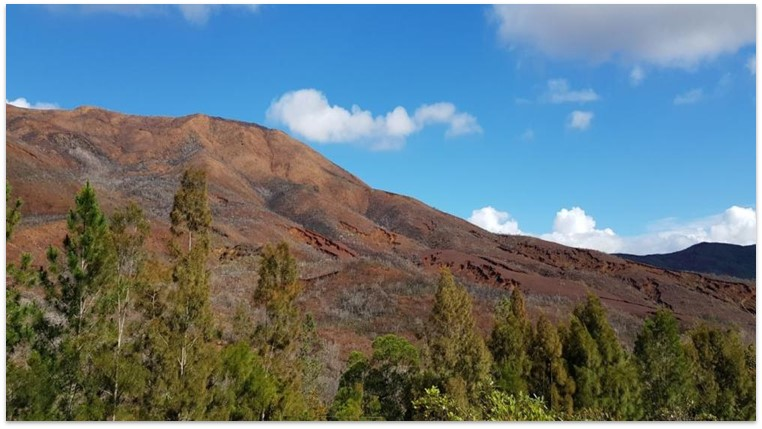
\includegraphics[width=27cm,height=16cm]{img/feux1.jpg}
        };
    \end{tikzpicture}

    %ajout de l'image supérieur
    \begin{tikzpicture}[remember picture, overlay]
        \clip [rounded corners=30pt] (-0.5cm,-2.5cm) rectangle ++(9cm,5.5cm);
        \node[inner sep=0pt, anchor=south west] at (-0.5cm,-2.5cm) { 
            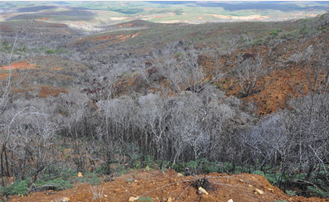
\includegraphics[width=10.5cm,height=6.5cm]{img/feux2.png}
        };
        \draw [white, line width=3pt, rounded corners=30pt] (-0.5cm,-2.5cm) rectangle ++(9cm,5.5cm); %trait blanc autour de l'image
    \end{tikzpicture}

% intégration des titre, sous-titre, auteurs et date
    \begin{minipage}[2cm]{16cm}
        \begin{adjustwidth}{-0.4cm}{1cm} 
            \vspace{3.2cm}
            {\fontsize{16}{20}\selectfont
            \color{titreColor}
            Contrôle des données en sortie de chaine INSIGHT\\
            }

            {\fontsize{12}{14}\selectfont
            \color{grey_color}
            Oriane Bruyère\\
            }
    
            {\fontsize{12}{8}\selectfont
            \color{date_color}
            février 2024\\
            }

        \end{adjustwidth}
    \end{minipage}

    %ajout du logo OEIL
    \begin{tikzpicture}[remember picture,overlay]
        \node [inner sep=0pt] at (12.5cm,-4.8cm) {\includegraphics[width=4.5cm,height=5.5cm]{img/OEIL\_logo.png} 
        };
    \end{tikzpicture}

    %ajout d'element supplémentaire ou logo partenaire
    \begin{minipage}[1cm]{16cm}
        \begin{adjustwidth}{-0.4cm}{1cm} 
            \vspace{3.4cm}
            {\fontsize{11}{13}\selectfont
            \color{version_color}
            Document technique - Diffusion interne à l'OEIL
            }
        \end{adjustwidth}
    \end{minipage}

\end{titlepage}

\renewcommand*\contentsname{Table des matières}
{
\hypersetup{linkcolor=}
\setcounter{tocdepth}{4}
\tableofcontents
}
\section{Start visual control}\label{start-visual-control}

\subsection{Présentation général des contrôles et leur incidence sur la
donnée
brute}\label{pruxe9sentation-guxe9nuxe9ral-des-contruxf4les-et-leur-incidence-sur-la-donnuxe9e-brute}

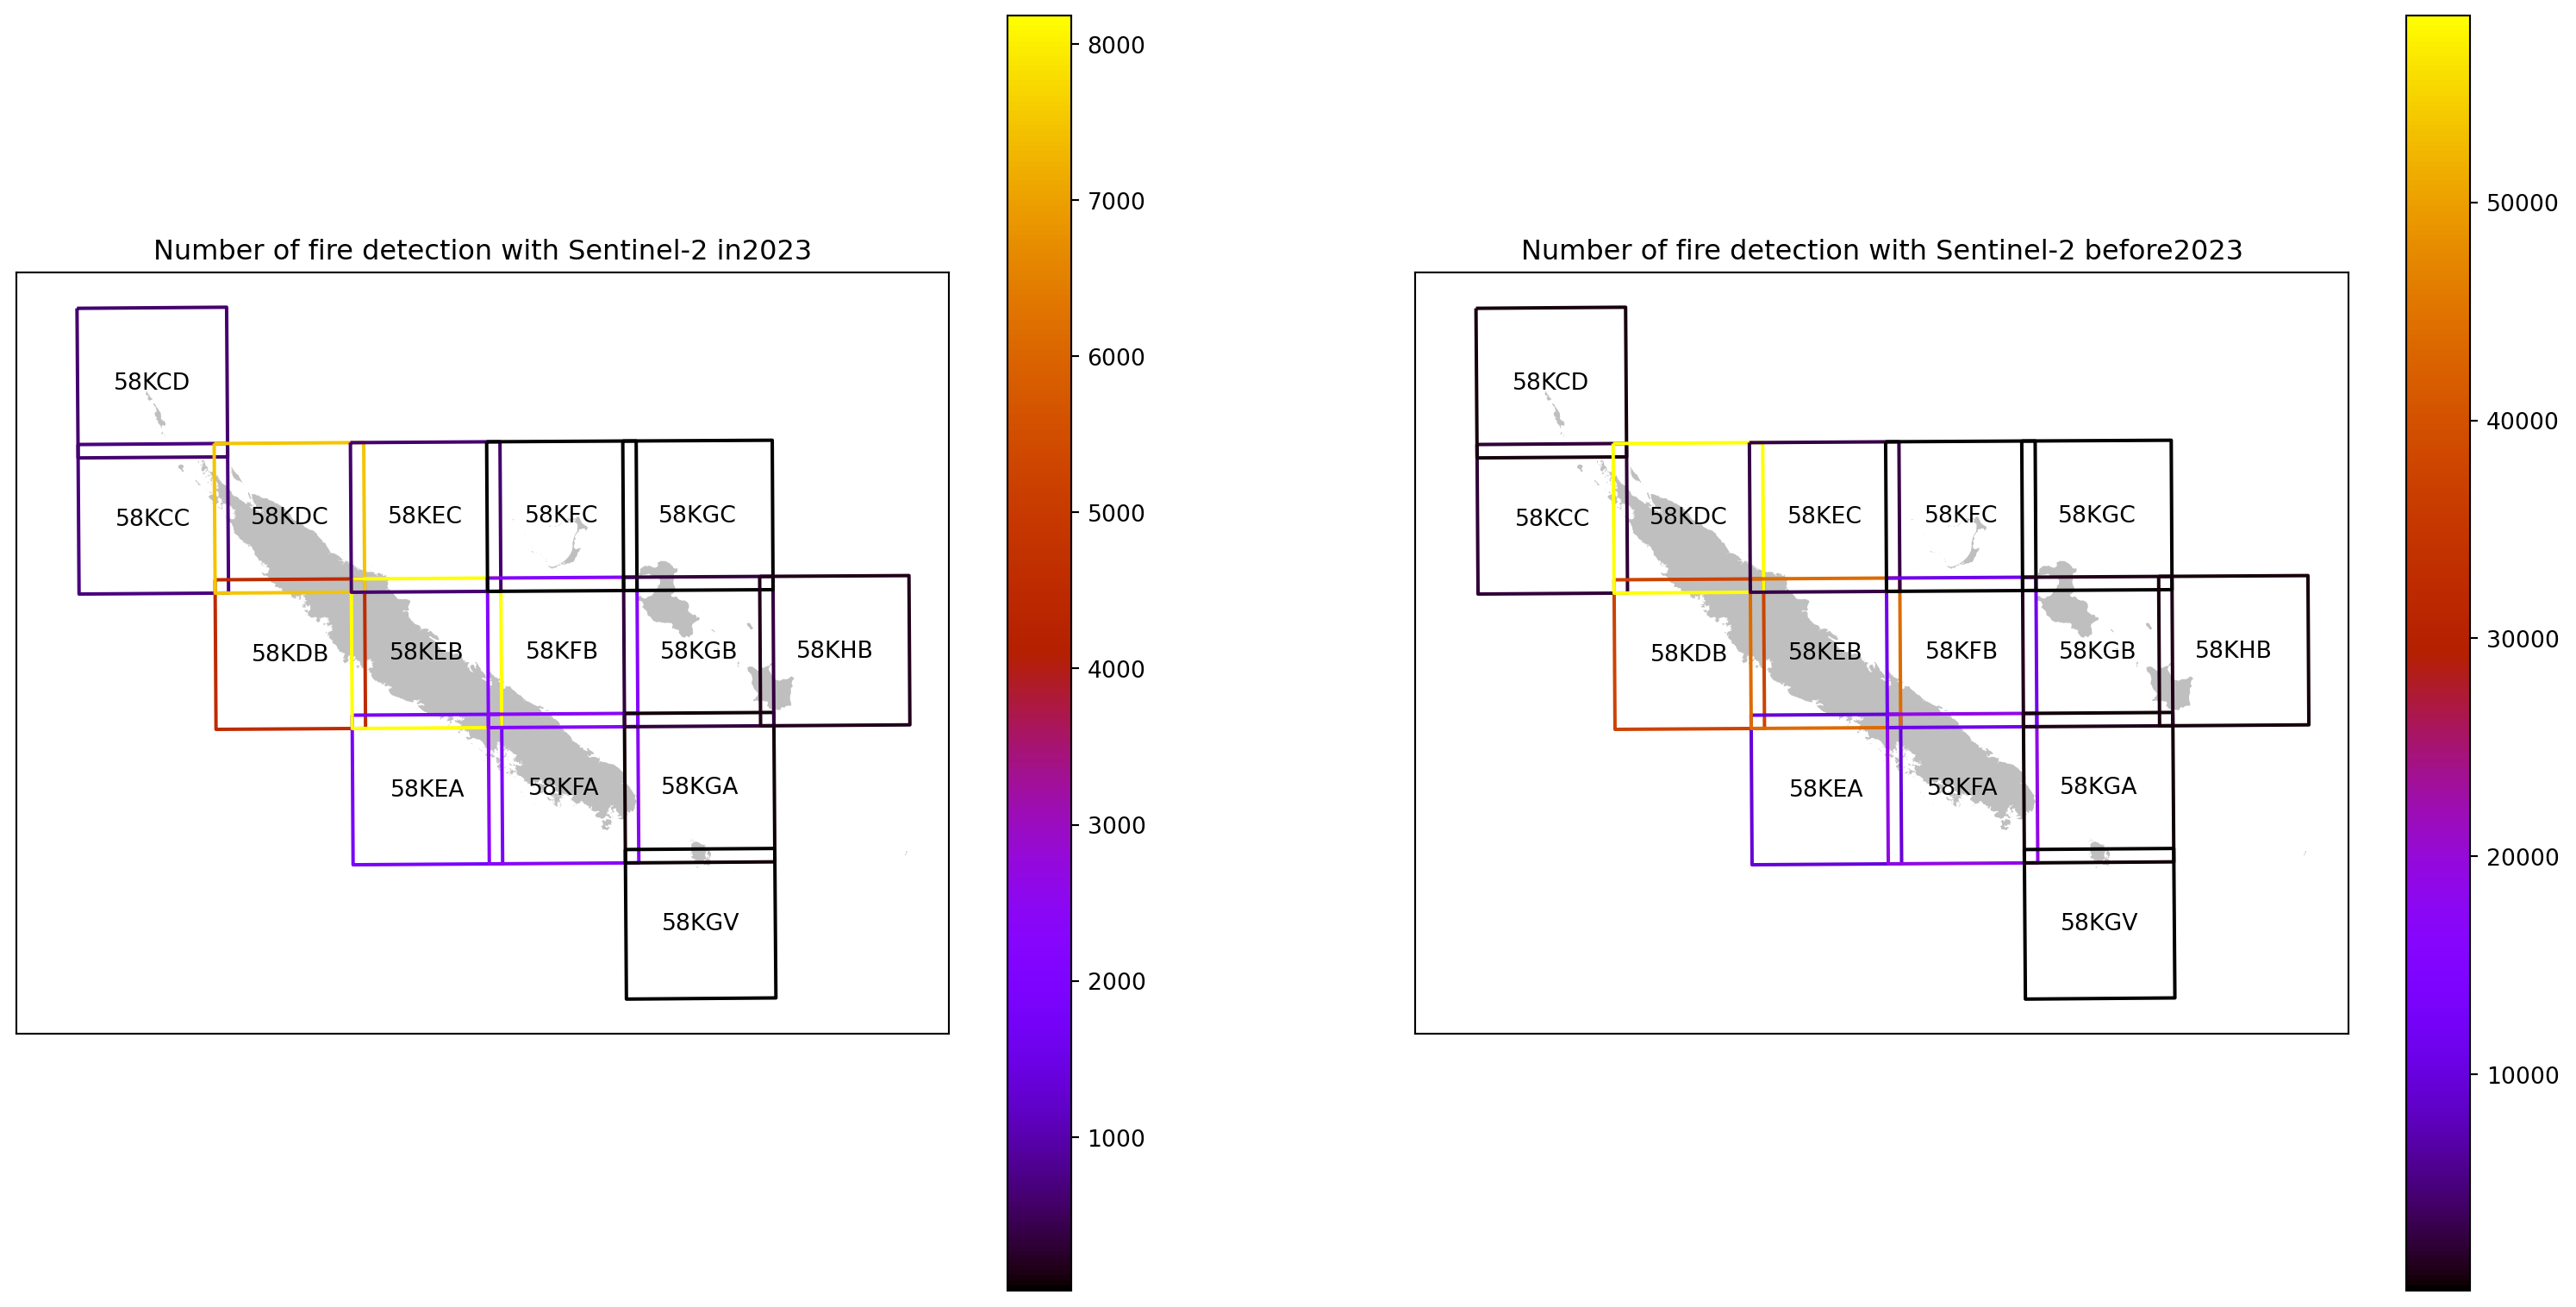
\includegraphics{control_data_quarto_files/figure-pdf/cell-3-output-1.pdf}



\end{document}
